\documentclass[11pt,a4paper,oneside]{ctexbook}

\usepackage{amsmath}
\usepackage{amssymb}
\usepackage{array}
\usepackage{booktabs}
\usepackage{calc}
\usepackage{caption}
\usepackage{changepage}

\usepackage{ctex}
\usepackage{ctexcap}
\usepackage{datetime}
% \usepackage{dingbat}

\usepackage{eurosym}
\usepackage{fancyhdr}

\usepackage{fontspec}
\usepackage{geometry}

\usepackage{glossaries}
\makeglossaries

\usepackage{graphicx}
\usepackage{graphpap}

\usepackage{ifthen}

\usepackage{listings}
\usepackage{longtable}

\usepackage{makeidx}
\makeindex

\usepackage{minted}
\usepackage{mflogo}

\usepackage{multicol}
\usepackage{multirow}

\usepackage{paralist}
\usepackage{pdflscape}

\usepackage{pgfornament}

\usepackage{svg}
\usepackage{syntonly}
\usepackage{tabularx}
\usepackage{textcomp}

\usepackage{tikz}
\usepackage{tracefnt}
\usepackage{ulem}
\usepackage{verbatim}

\usepackage{xcolor}

\usepackage{hyperref}
\usetikzlibrary{shapes}


\bibliographystyle{plain}


\hypersetup{
	hidelinks,
	baseurl=https://github.com/hiatcg,
	pdftitle=随手笔记,
	pdfauthor=张洋,
	pdfsubject={随手笔记},
	pdfkeywords={随手笔记},
	pdfstartview=FitH,
	pdfcreator=hiatcg,
	pdfproducer=hiatcg,
	pdfcenterwindow=true
}

\begin{document}
	\tableofcontents
	\input{./auto_combine}

\chapter{The Neural Network Zoo}

With new neural network architectures popping up every now and then, it’s hard to keep track of them all. Knowing all the abbreviations being thrown around (DCIGN, BiLSTM, DCGAN, anyone?) can be a bit overwhelming at first.

So I decided to compose a cheat sheet containing many of those architectures. Most of these are neural networks, some are completely different beasts. Though all of these architectures are presented as novel and unique, when I drew the node structures… their underlying relations started to make more sense.

\begin{figure}
	\centering
	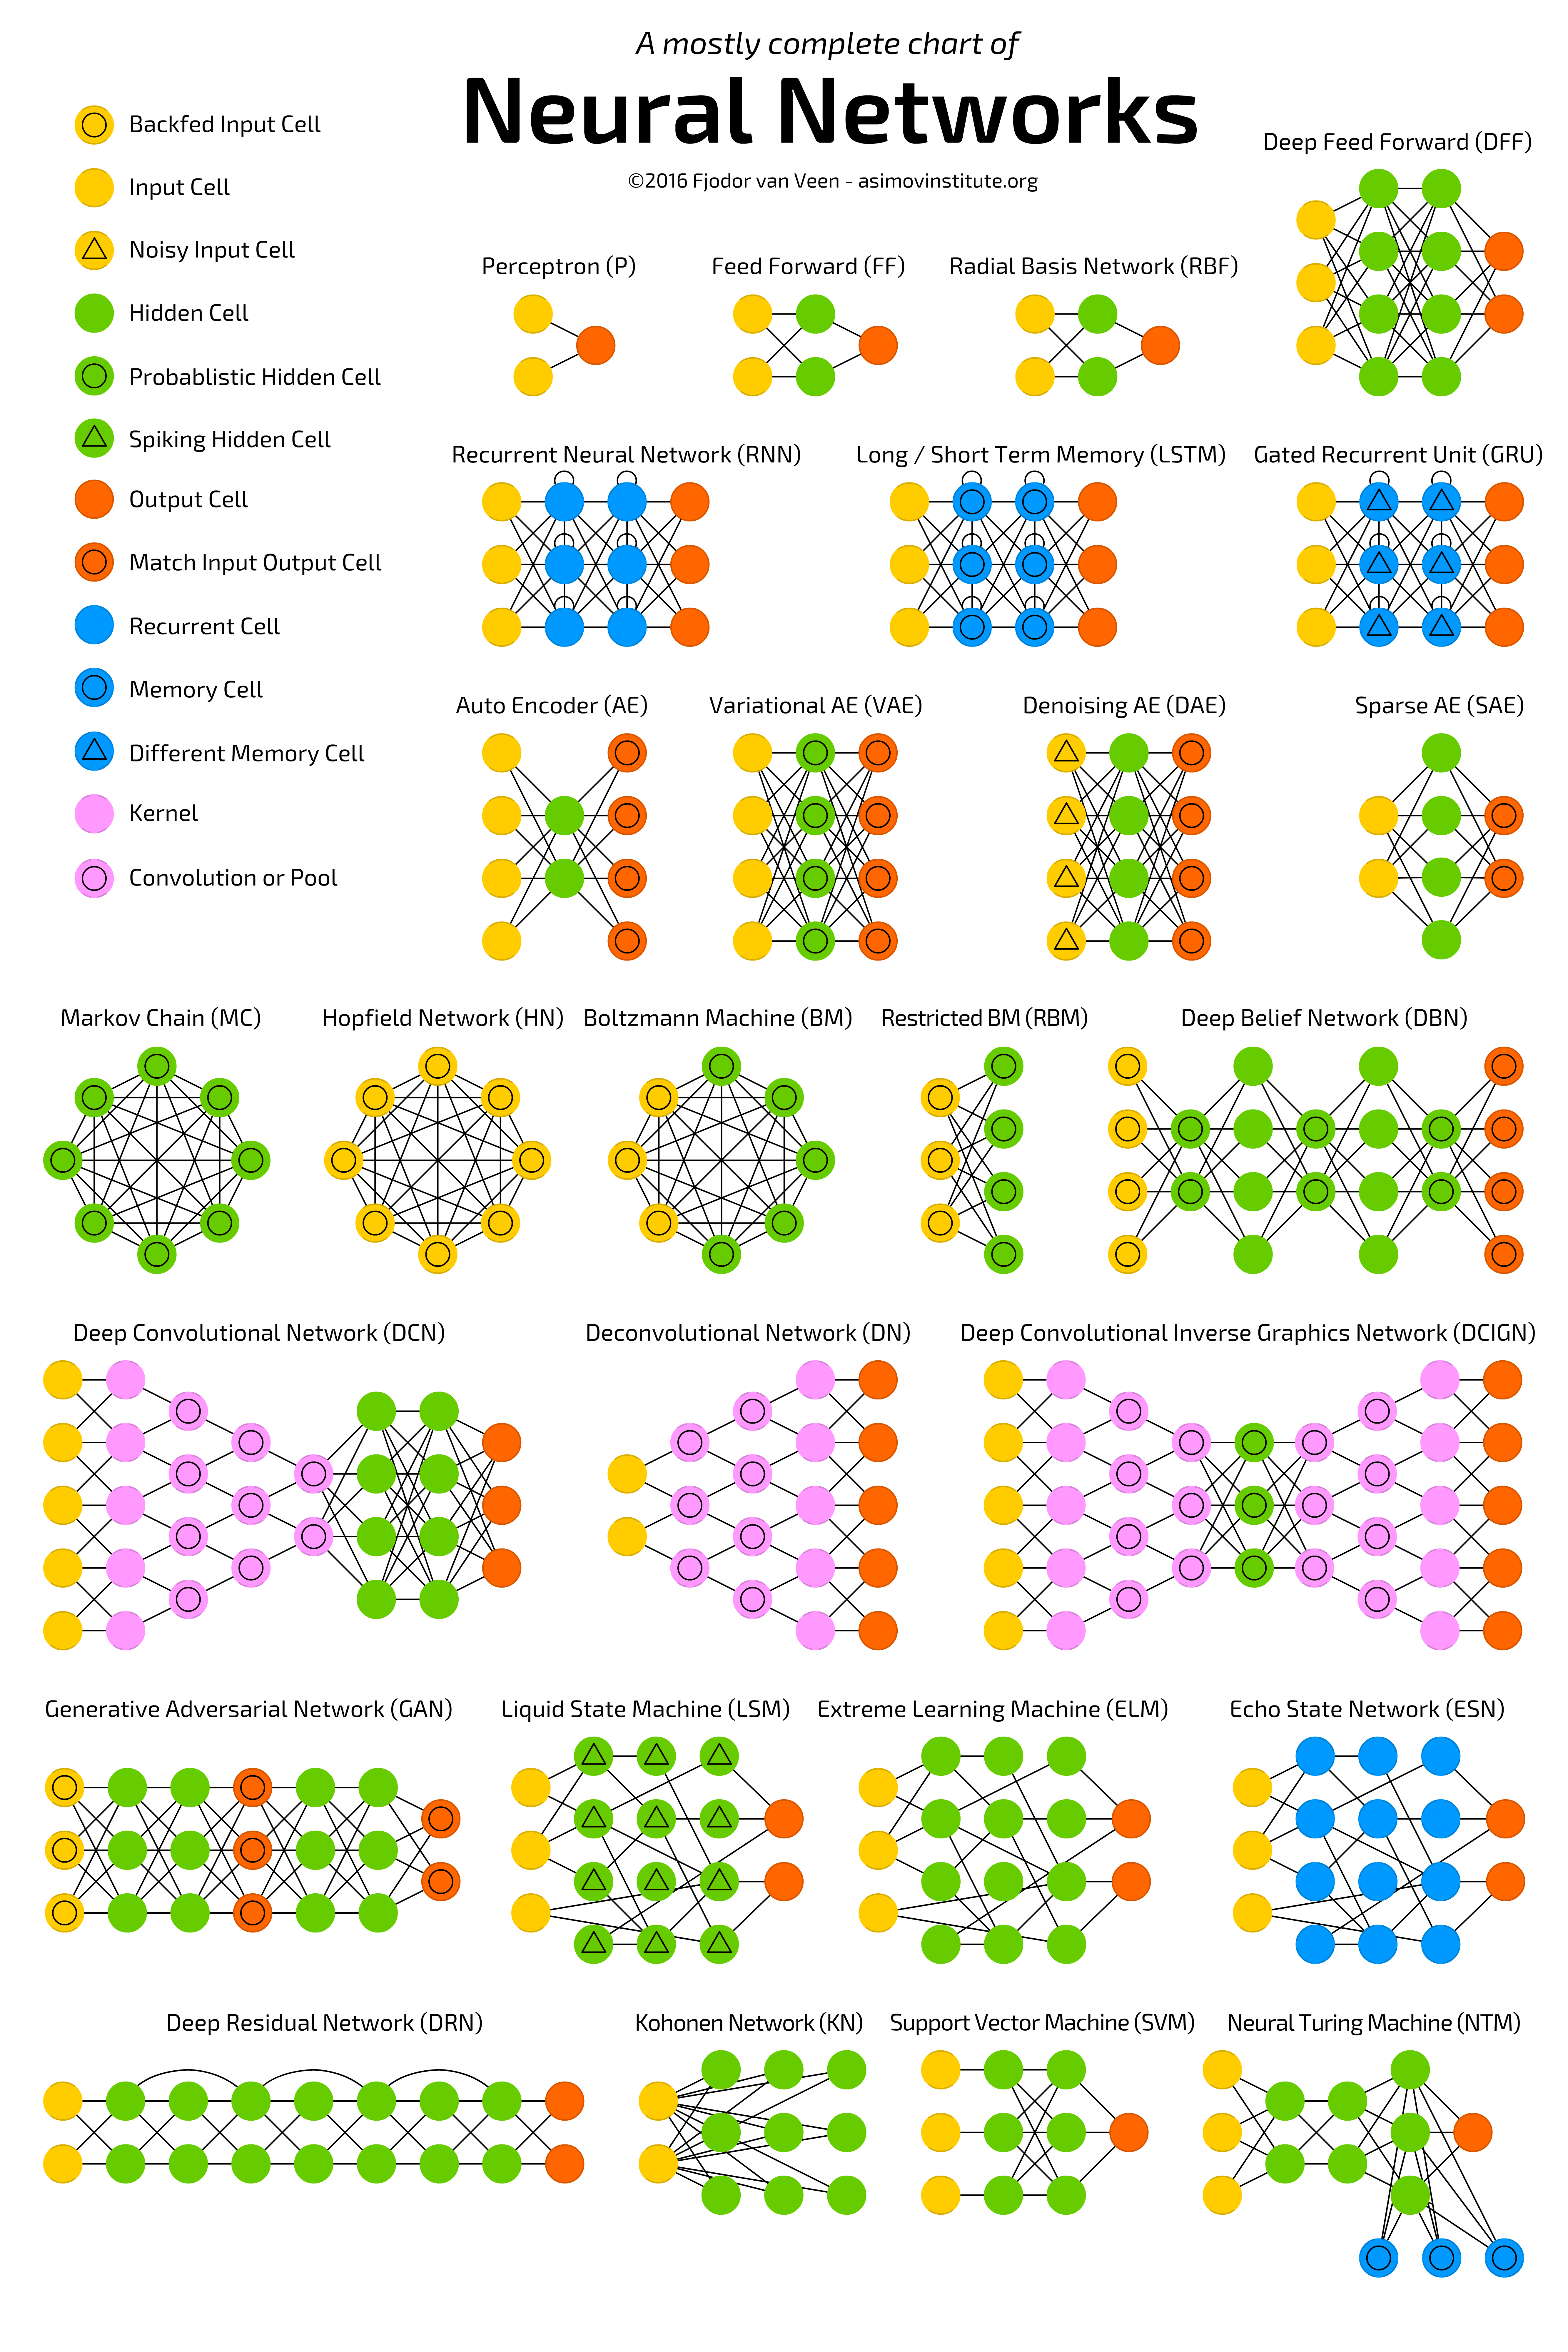
\includegraphics[width=\linewidth]{figures/neuralnetworks}
	\caption{A Mostly Complete Chart of Neural Networks}
	\label{fig:neuralnetworks}
\end{figure}


One problem with drawing them as node maps: it doesn’t really show how they’re used. For example, variational autoencoders (VAE) may look just like autoencoders (AE), but the training process is actually quite different. The use-cases for trained networks differ even more, because VAEs are generators, where you insert noise to get a new sample. AEs, simply map whatever they get as input to the closest training sample they “remember”. I should add that this overview is in no way clarifying how each of the different node types work internally (but that’s a topic for another day).

It should be noted that while most of the abbreviations used are generally accepted, not all of them are. RNNs sometimes refer to recursive neural networks, but most of the time they refer to recurrent neural networks. That’s not the end of it though, in many places you’ll find RNN used as placeholder for any recurrent architecture, including LSTMs, GRUs and even the bidirectional variants. AEs suffer from a similar problem from time to time, where VAEs and DAEs and the like are called simply AEs. Many abbreviations also vary in the amount of “N”s to add at the end, because you could call it a convolutional neural network but also simply a convolutional network (resulting in CNN or CN).

Composing a complete list is practically impossible, as new architectures are invented all the time. Even if published it can still be quite challenging to find them even if you’re looking for them, or sometimes you just overlook some. So while this list may provide you with some insights into the world of AI, please, by no means take this list for being comprehensive; especially if you read this post long after it was written.

For each of the architectures depicted in the picture, I wrote a very, very brief description. You may find some of these to be useful if you’re quite familiar with some architectures, but you aren’t familiar with a particular one.
	
	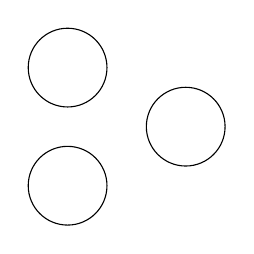
\begin{tikzpicture}
	\draw (0,0) circle [radius=0.5];
	\draw (0,1.5) circle [radius=0.5];
	\draw (1.5,0.75) circle [radius=0.5];
	\end{tikzpicture}

\begin{figure}
	\centering
	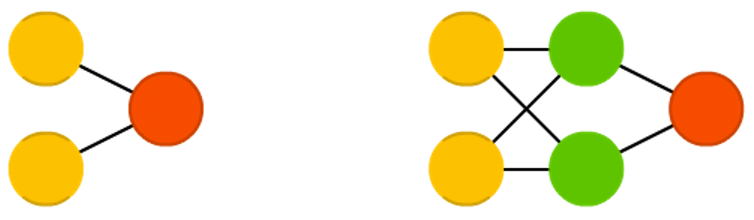
\includegraphics{figures/ff}
	\caption{}
	\label{fig:ff}
\end{figure}

Feed forward neural networks (FF or FFNN) and perceptrons (P) are very straight forward, they feed information from the front to the back (input and output, respectively). Neural networks are often described as having layers, where each layer consists of either input, hidden or output cells in parallel. A layer alone never has connections and in general two adjacent layers are fully connected (every neuron form one layer to every neuron to another layer). The simplest somewhat practical network has two input cells and one output cell, which can be used to model logic gates. One usually trains FFNNs through back-propagation, giving the network paired datasets of “what goes in” and “what we want to have coming out”. This is called supervised learning, as opposed to unsupervised learning where we only give it input and let the network fill in the blanks. The error being back-propagated is often some variation of the difference between the input and the output (like MSE or just the linear difference). Given that the network has enough hidden neurons, it can theoretically always model the relationship between the input and output. Practically their use is a lot more limited but they are popularly combined with other networks to form new networks.
Rosenblatt, Frank. “The perceptron: a probabilistic model for information storage and organization in the brain.” Psychological review 65.6 (1958): 386.
Original Paper PDF


Radial basis function (RBF) networks are FFNNs with radial basis functions as activation functions. There’s nothing more to it. Doesn’t mean they don’t have their uses, but most FFNNs with other activation functions don’t get their own name. This mostly has to do with inventing them at the right time.
Broomhead, David S., and David Lowe. Radial basis functions, multi-variable functional interpolation and adaptive networks. No. RSRE-MEMO-4148. ROYAL SIGNALS AND RADAR ESTABLISHMENT MALVERN (UNITED KINGDOM), 1988.
Original Paper PDF


A Hopfield network (HN) is a network where every neuron is connected to every other neuron; it is a completely entangled plate of spaghetti as even all the nodes function as everything. Each node is input before training, then hidden during training and output afterwards. The networks are trained by setting the value of the neurons to the desired pattern after which the weights can be computed. The weights do not change after this. Once trained for one or more patterns, the network will always converge to one of the learned patterns because the network is only stable in those states. Note that it does not always conform to the desired state (it’s not a magic black box sadly). It stabilises in part due to the total “energy” or “temperature” of the network being reduced incrementally during training. Each neuron has an activation threshold which scales to this temperature, which if surpassed by summing the input causes the neuron to take the form of one of two states (usually -1 or 1, sometimes 0 or 1). Updating the network can be done synchronously or more commonly one by one. If updated one by one, a fair random sequence is created to organise which cells update in what order (fair random being all options (n) occurring exactly once every n items). This is so you can tell when the network is stable (done converging), once every cell has been updated and none of them changed, the network is stable (annealed). These networks are often called associative memory because the converge to the most similar state as the input; if humans see half a table we can image the other half, this network will converge to a table if presented with half noise and half a table.
Hopfield, John J. “Neural networks and physical systems with emergent collective computational abilities.” Proceedings of the national academy of sciences 79.8 (1982): 2554-2558.
Original Paper PDF


Markov chains (MC or discrete time Markov Chain, DTMC) are kind of the predecessors to BMs and HNs. They can be understood as follows: from this node where I am now, what are the odds of me going to any of my neighbouring nodes? They are memoryless (i.e. Markov Property) which means that every state you end up in depends completely on the previous state. While not really a neural network, they do resemble neural networks and form the theoretical basis for BMs and HNs. MC aren’t always considered neural networks, as goes for BMs, RBMs and HNs. Markov chains aren’t always fully connected either.
Hayes, Brian. “First links in the Markov chain.” American Scientist 101.2 (2013): 252.
Original Paper PDF


Boltzmann machines (BM) are a lot like HNs, but: some neurons are marked as input neurons and others remain “hidden”. The input neurons become output neurons at the end of a full network update. It starts with random weights and learns through back-propagation, or more recently through contrastive divergence (a Markov chain is used to determine the gradients between two informational gains). Compared to a HN, the neurons mostly have binary activation patterns. As hinted by being trained by MCs, BMs are stochastic networks. The training and running process of a BM is fairly similar to a HN: one sets the input neurons to certain clamped values after which the network is set free (it doesn’t get a sock). While free the cells can get any value and we repetitively go back and forth between the input and hidden neurons. The activation is controlled by a global temperature value, which if lowered lowers the energy of the cells. This lower energy causes their activation patterns to stabilise. The network reaches an equilibrium given the right temperature.
Hinton, Geoffrey E., and Terrence J. Sejnowski. “Learning and releaming in Boltzmann machines.” Parallel distributed processing: Explorations in the microstructure of cognition 1 (1986): 282-317.
Original Paper PDF


Restricted Boltzmann machines (RBM) are remarkably similar to BMs (surprise) and therefore also similar to HNs. The biggest difference between BMs and RBMs is that RBMs are a better usable because they are more restricted. They don’t trigger-happily connect every neuron to every other neuron but only connect every different group of neurons to every other group, so no input neurons are directly connected to other input neurons and no hidden to hidden connections are made either. RBMs can be trained like FFNNs with a twist: instead of passing data forward and then back-propagating, you forward pass the data and then backward pass the data (back to the first layer). After that you train with forward-and-back-propagation.
Smolensky, Paul. Information processing in dynamical systems: Foundations of harmony theory. No. CU-CS-321-86. COLORADO UNIV AT BOULDER DEPT OF COMPUTER SCIENCE, 1986.
Original Paper PDF


Autoencoders (AE) are somewhat similar to FFNNs as AEs are more like a different use of FFNNs than a fundamentally different architecture. The basic idea behind autoencoders is to encode information (as in compress, not encrypt) automatically, hence the name. The entire network always resembles an hourglass like shape, with smaller hidden layers than the input and output layers. AEs are also always symmetrical around the middle layer(s) (one or two depending on an even or odd amount of layers). The smallest layer(s) is|are almost always in the middle, the place where the information is most compressed (the chokepoint of the network). Everything up to the middle is called the encoding part, everything after the middle the decoding and the middle (surprise) the code. One can train them using backpropagation by feeding input and setting the error to be the difference between the input and what came out. AEs can be built symmetrically when it comes to weights as well, so the encoding weights are the same as the decoding weights.
Bourlard, Hervé, and Yves Kamp. “Auto-association by multilayer perceptrons and singular value decomposition.” Biological cybernetics 59.4-5 (1988): 291-294.
Original Paper PDF


Sparse autoencoders (SAE) are in a way the opposite of AEs. Instead of teaching a network to represent a bunch of information in less “space” or nodes, we try to encode information in more space. So instead of the network converging in the middle and then expanding back to the input size, we blow up the middle. These types of networks can be used to extract many small features from a dataset. If one were to train a SAE the same way as an AE, you would in almost all cases end up with a pretty useless identity network (as in what comes in is what comes out, without any transformation or decomposition). To prevent this, instead of feeding back the input, we feed back the input plus a sparsity driver. This sparsity driver can take the form of a threshold filter, where only a certain error is passed back and trained, the other error will be “irrelevant” for that pass and set to zero. In a way this resembles spiking neural networks, where not all neurons fire all the time (and points are scored for biological plausibility).
Marc’Aurelio Ranzato, Christopher Poultney, Sumit Chopra, and Yann LeCun. “Efficient learning of sparse representations with an energy-based model.” Proceedings of NIPS. 2007.
Original Paper PDF


Variational autoencoders (VAE) have the same architecture as AEs but are “taught” something else: an approximated probability distribution of the input samples. It’s a bit back to the roots as they are bit more closely related to BMs and RBMs. They do however rely on Bayesian mathematics regarding probabilistic inference and independence, as well as a re-parametrisation trick to achieve this different representation. The inference and independence parts make sense intuitively, but they rely on somewhat complex mathematics. The basics come down to this: take influence into account. If one thing happens in one place and something else happens somewhere else, they are not necessarily related. If they are not related, then the error propagation should consider that. This is a useful approach because neural networks are large graphs (in a way), so it helps if you can rule out influence from some nodes to other nodes as you dive into deeper layers.
Kingma, Diederik P., and Max Welling. “Auto-encoding variational bayes.” arXiv preprint arXiv:1312.6114 (2013).
Original Paper PDF


Denoising autoencoders (DAE) are AEs where we don’t feed just the input data, but we feed the input data with noise (like making an image more grainy). We compute the error the same way though, so the output of the network is compared to the original input without noise. This encourages the network not to learn details but broader features, as learning smaller features often turns out to be “wrong” due to it constantly changing with noise.
Vincent, Pascal, et al. “Extracting and composing robust features with denoising autoencoders.” Proceedings of the 25th international conference on Machine learning. ACM, 2008.
Original Paper PDF


Deep belief networks (DBN) is the name given to stacked architectures of mostly RBMs or VAEs. These networks have been shown to be effectively trainable stack by stack, where each AE or RBM only has to learn to encode the previous network. This technique is also known as greedy training, where greedy means making locally optimal solutions to get to a decent but possibly not optimal answer. DBNs can be trained through contrastive divergence or back-propagation and learn to represent the data as a probabilistic model, just like regular RBMs or VAEs. Once trained or converged to a (more) stable state through unsupervised learning, the model can be used to generate new data. If trained with contrastive divergence, it can even classify existing data because the neurons have been taught to look for different features.
Bengio, Yoshua, et al. “Greedy layer-wise training of deep networks.” Advances in neural information processing systems 19 (2007): 153.
Original Paper PDF


Convolutional neural networks (CNN or deep convolutional neural networks, DCNN) are quite different from most other networks. They are primarily used for image processing but can also be used for other types of input such as as audio. A typical use case for CNNs is where you feed the network images and the network classifies the data, e.g. it outputs “cat” if you give it a cat picture and “dog” when you give it a dog picture. CNNs tend to start with an input “scanner” which is not intended to parse all the training data at once. For example, to input an image of 200 x 200 pixels, you wouldn’t want a layer with 40 000 nodes. Rather, you create a scanning input layer of say 20 x 20 which you feed the first 20 x 20 pixels of the image (usually starting in the upper left corner). Once you passed that input (and possibly use it for training) you feed it the next 20 x 20 pixels: you move the scanner one pixel to the right. Note that one wouldn’t move the input 20 pixels (or whatever scanner width) over, you’re not dissecting the image into blocks of 20 x 20, but rather you’re crawling over it. This input data is then fed through convolutional layers instead of normal layers, where not all nodes are connected to all nodes. Each node only concerns itself with close neighbouring cells (how close depends on the implementation, but usually not more than a few). These convolutional layers also tend to shrink as they become deeper, mostly by easily divisible factors of the input (so 20 would probably go to a layer of 10 followed by a layer of 5). Powers of two are very commonly used here, as they can be divided cleanly and completely by definition: 32, 16, 8, 4, 2, 1. Besides these convolutional layers, they also often feature pooling layers. Pooling is a way to filter out details: a commonly found pooling technique is max pooling, where we take say 2 x 2 pixels and pass on the pixel with the most amount of red. To apply CNNs for audio, you basically feed the input audio waves and inch over the length of the clip, segment by segment. Real world implementations of CNNs often glue an FFNN to the end to further process the data, which allows for highly non-linear abstractions. These networks are called DCNNs but the names and abbreviations between these two are often used interchangeably.
LeCun, Yann, et al. “Gradient-based learning applied to document recognition.” Proceedings of the IEEE 86.11 (1998): 2278-2324.
Original Paper PDF


Deconvolutional networks (DN), also called inverse graphics networks (IGNs), are reversed convolutional neural networks. Imagine feeding a network the word “cat” and training it to produce cat-like pictures, by comparing what it generates to real pictures of cats. DNNs can be combined with FFNNs just like regular CNNs, but this is about the point where the line is drawn with coming up with new abbreviations. They may be referenced as deep deconvolutional neural networks, but you could argue that when you stick FFNNs to the back and the front of DNNs that you have yet another architecture which deserves a new name. Note that in most applications one wouldn’t actually feed text-like input to the network, more likely a binary classification input vector. Think <0, 1> being cat, <1, 0> being dog and <1, 1> being cat and dog. The pooling layers commonly found in CNNs are often replaced with similar inverse operations, mainly interpolation and extrapolation with biased assumptions (if a pooling layer uses max pooling, you can invent exclusively lower new data when reversing it).
Zeiler, Matthew D., et al. “Deconvolutional networks.” Computer Vision and Pattern Recognition (CVPR), 2010 IEEE Conference on. IEEE, 2010.
Original Paper PDF


Deep convolutional inverse graphics networks (DCIGN) have a somewhat misleading name, as they are actually VAEs but with CNNs and DNNs for the respective encoders and decoders. These networks attempt to model “features” in the encoding as probabilities, so that it can learn to produce a picture with a cat and a dog together, having only ever seen one of the two in separate pictures. Similarly, you could feed it a picture of a cat with your neighbours’ annoying dog on it, and ask it to remove the dog, without ever having done such an operation. Demo’s have shown that these networks can also learn to model complex transformations on images, such as changing the source of light or the rotation of a 3D object. These networks tend to be trained with back-propagation.
Kulkarni, Tejas D., et al. “Deep convolutional inverse graphics network.” Advances in Neural Information Processing Systems. 2015.
Original Paper PDF


Generative adversarial networks (GAN) are from a different breed of networks, they are twins: two networks working together. GANs consist of any two networks (although often a combination of FFs and CNNs), with one tasked to generate content and the other has to judge content. The discriminating network receives either training data or generated content from the generative network. How well the discriminating network was able to correctly predict the data source is then used as part of the error for the generating network. This creates a form of competition where the discriminator is getting better at distinguishing real data from generated data and the generator is learning to become less predictable to the discriminator. This works well in part because even quite complex noise-like patterns are eventually predictable but generated content similar in features to the input data is harder to learn to distinguish. GANs can be quite difficult to train, as you don’t just have to train two networks (either of which can pose it’s own problems) but their dynamics need to be balanced as well. If prediction or generation becomes to good compared to the other, a GAN won’t converge as there is intrinsic divergence.
Goodfellow, Ian, et al. “Generative adversarial nets.” Advances in Neural Information Processing Systems. 2014.
Original Paper PDF


Recurrent neural networks (RNN) are FFNNs with a time twist: they are not stateless; they have connections between passes, connections through time. Neurons are fed information not just from the previous layer but also from themselves from the previous pass. This means that the order in which you feed the input and train the network matters: feeding it “milk” and then “cookies” may yield different results compared to feeding it “cookies” and then “milk”. One big problem with RNNs is the vanishing (or exploding) gradient problem where, depending on the activation functions used, information rapidly gets lost over time, just like very deep FFNNs lose information in depth. Intuitively this wouldn’t be much of a problem because these are just weights and not neuron states, but the weights through time is actually where the information from the past is stored; if the weight reaches a value of 0 or 1 000 000, the previous state won’t be very informative. RNNs can in principle be used in many fields as most forms of data that don’t actually have a timeline (i.e. unlike sound or video) can be represented as a sequence. A picture or a string of text can be fed one pixel or character at a time, so the time dependent weights are used for what came before in the sequence, not actually from what happened x seconds before. In general, recurrent networks are a good choice for advancing or completing information, such as autocompletion.
Elman, Jeffrey L. “Finding structure in time.” Cognitive science 14.2 (1990): 179-211.
Original Paper PDF


Long / short term memory (LSTM) networks try to combat the vanishing / exploding gradient problem by introducing gates and an explicitly defined memory cell. These are inspired mostly by circuitry, not so much biology. Each neuron has a memory cell and three gates: input, output and forget. The function of these gates is to safeguard the information by stopping or allowing the flow of it. The input gate determines how much of the information from the previous layer gets stored in the cell. The output layer takes the job on the other end and determines how much of the next layer gets to know about the state of this cell. The forget gate seems like an odd inclusion at first but sometimes it’s good to forget: if it’s learning a book and a new chapter begins, it may be necessary for the network to forget some characters from the previous chapter. LSTMs have been shown to be able to learn complex sequences, such as writing like Shakespeare or composing primitive music. Note that each of these gates has a weight to a cell in the previous neuron, so they typically require more resources to run.
Hochreiter, Sepp, and Jürgen Schmidhuber. “Long short-term memory.” Neural computation 9.8 (1997): 1735-1780.
Original Paper PDF


Gated recurrent units (GRU) are a slight variation on LSTMs. They have one less gate and are wired slightly differently: instead of an input, output and a forget gate, they have an update gate. This update gate determines both how much information to keep from the last state and how much information to let in from the previous layer. The reset gate functions much like the forget gate of an LSTM but it’s located slightly differently. They always send out their full state, they don’t have an output gate. In most cases, they function very similarly to LSTMs, with the biggest difference being that GRUs are slightly faster and easier to run (but also slightly less expressive). In practice these tend to cancel each other out, as you need a bigger network to regain some expressiveness which then in turn cancels out the performance benefits. In some cases where the extra expressiveness is not needed, GRUs can outperform LSTMs.
Chung, Junyoung, et al. “Empirical evaluation of gated recurrent neural networks on sequence modeling.” arXiv preprint arXiv:1412.3555 (2014).
Original Paper PDF



Neural Turing machines (NTM) can be understood as an abstraction of LSTMs and an attempt to un-black-box neural networks (and give us some insight in what is going on in there). Instead of coding a memory cell directly into a neuron, the memory is separated. It’s an attempt to combine the efficiency and permanency of regular digital storage and the efficiency and expressive power of neural networks. The idea is to have a content-addressable memory bank and a neural network that can read and write from it. The “Turing” in Neural Turing Machines comes from them being Turing complete: the ability to read and write and change state based on what it reads means it can represent anything a Universal Turing Machine can represent.
Graves, Alex, Greg Wayne, and Ivo Danihelka. “Neural turing machines.” arXiv preprint arXiv:1410.5401 (2014).
Original Paper PDF

Bidirectional recurrent neural networks, bidirectional long / short term memory networks and bidirectional gated recurrent units (BiRNN, BiLSTM and BiGRU respectively) are not shown on the chart because they look exactly the same as their unidirectional counterparts. The difference is that these networks are not just connected to the past, but also to the future. As an example, unidirectional LSTMs might be trained to predict the word “fish” by being fed the letters one by one, where the recurrent connections through time remember the last value. A BiLSTM would also be fed the next letter in the sequence on the backward pass, giving it access to future information. This trains the network to fill in gaps instead of advancing information, so instead of expanding an image on the edge, it could fill a hole in the middle of an image.
Schuster, Mike, and Kuldip K. Paliwal. “Bidirectional recurrent neural networks.” IEEE Transactions on Signal Processing 45.11 (1997): 2673-2681.
Original Paper PDF


Deep residual networks (DRN) are very deep FFNNs with extra connections passing input from one layer to a later layer (often 2 to 5 layers) as well as the next layer. Instead of trying to find a solution for mapping some input to some output across say 5 layers, the network is enforced to learn to map some input to some output + some input. Basically, it adds an identity to the solution, carrying the older input over and serving it freshly to a later layer. It has been shown that these networks are very effective at learning patterns up to 150 layers deep, much more than the regular 2 to 5 layers one could expect to train. However, it has been proven that these networks are in essence just RNNs without the explicit time based construction and they’re often compared to LSTMs without gates.
He, Kaiming, et al. “Deep residual learning for image recognition.” arXiv preprint arXiv:1512.03385 (2015).
Original Paper PDF


Echo state networks (ESN) are yet another different type of (recurrent) network. This one sets itself apart from others by having random connections between the neurons (i.e. not organised into neat sets of layers), and they are trained differently. Instead of feeding input and back-propagating the error, we feed the input, forward it and update the neurons for a while, and observe the output over time. The input and the output layers have a slightly unconventional role as the input layer is used to prime the network and the output layer acts as an observer of the activation patterns that unfold over time. During training, only the connections between the observer and the (soup of) hidden units are changed.
Jaeger, Herbert, and Harald Haas. “Harnessing nonlinearity: Predicting chaotic systems and saving energy in wireless communication.” science 304.5667 (2004): 78-80.
Original Paper PDF


Extreme learning machines (ELM) are basically FFNNs but with random connections. They look very similar to LSMs and ESNs, but they are not recurrent nor spiking. They also do not use backpropagation. Instead, they start with random weights and train the weights in a single step according to the least-squares fit (lowest error across all functions). This results in a much less expressive network but it’s also much faster than backpropagation.
Cambria, Erik, et al. “Extreme learning machines [trends \& controversies].” IEEE Intelligent Systems 28.6 (2013): 30-59.
Original Paper PDF


Liquid state machines (LSM) are similar soups, looking a lot like ESNs. The real difference is that LSMs are a type of spiking neural networks: sigmoid activations are replaced with threshold functions and each neuron is also an accumulating memory cell. So when updating a neuron, the value is not set to the sum of the neighbours, but rather added to itself. Once the threshold is reached, it releases its’ energy to other neurons. This creates a spiking like pattern, where nothing happens for a while until a threshold is suddenly reached.
Maass, Wolfgang, Thomas Natschläger, and Henry Markram. “Real-time computing without stable states: A new framework for neural computation based on perturbations.” Neural computation 14.11 (2002): 2531-2560.
Original Paper PDF


Support vector machines (SVM) find optimal solutions for classification problems. Classically they were only capable of categorising linearly separable data; say finding which images are of Garfield and which of Snoopy, with any other outcome not being possible. During training, SVMs can be thought of as plotting all the data (Garfields and Snoopys) on a graph (2D) and figuring out how to draw a line between the data points. This line would separate the data, so that all Snoopys are on one side and the Garfields on the other. This line moves to an optimal line in such a way that the margins between the data points and the line are maximised on both sides. Classifying new data would be done by plotting a point on this graph and simply looking on which side of the line it is (Snoopy side or Garfield side). Using the kernel trick, they can be taught to classify n-dimensional data. This entails plotting points in a 3D plot, allowing it to distinguish between Snoopy, Garfield AND Simon’s cat, or even higher dimensions distinguishing even more cartoon characters. SVMs are not always considered neural networks.
Cortes, Corinna, and Vladimir Vapnik. “Support-vector networks.” Machine learning 20.3 (1995): 273-297.
Original Paper PDF


And finally, Kohonen networks (KN, also self organising (feature) map, SOM, SOFM) “complete” our zoo. KNs utilise competitive learning to classify data without supervision. Input is presented to the network, after which the network assesses which of its neurons most closely match that input. These neurons are then adjusted to match the input even better, dragging along their neighbours in the process. How much the neighbours are moved depends on the distance of the neighbours to the best matching units. KNs are sometimes not considered neural networks either.
Kohonen, Teuvo. “Self-organized formation of topologically correct feature maps.” Biological cybernetics 43.1 (1982): 59-69.
Original Paper PDF

Any feedback and criticism is welcome. At the Asimov Institute we do deep learning research and development, so be sure to follow us on twitter for future updates and posts! Thank you for reading!
[UPDATE 15 sept 2016] I would like to thank everybody for their insights and corrections, all feedback is hugely appreciated. I will add links and a couple more suggested networks in a future update, stay tuned.
[UPDATE 29 sept 2016] Added links and citations to all the original papers. A follow up post is planned, since I found at least 9 more architectures. I will not include them in this post for better consistency in terms of content.
Click here for a high res version of the full image.

\end{document}